\documentclass[10pt]{beamer}

%%%
% PREAMBLE FOR THIS DOC 
%%%
%https://tex.stackexchange.com/questions/68821/is-it-possible-to-create-a-latex-preamble-header
\usepackage{/Users/miw267/Repos/csci246_spring2025/slides/preambles/beamer_preamble_for_CSCI246}

\usetikzlibrary{matrix}


%%% TRY TO RESHOW TOC AT EACH SECTION START (with current section highlighted)
% Reference: https://tex.stackexchange.com/questions/280436/how-to-highlight-a-specific-section-in-beamer-toc
\newcommand\tocforsect[2]{%
  \begingroup
  \edef\safesection{\thesection}
  \setcounter{section}{#1}
  \tableofcontents[#2,currentsection]
  \setcounter{section}{\safesection}
  \endgroup
}


%%%% HERES HOW TO DO IT CORRECTLY
% FIRST IN .STY FILE, DO
%\usetheme[sectionpage=none]{metropolis}
% THEN AT EACH SECTION DO
%\begin{frame}{Outline}
%  \tableofcontents[currentsection]	
%\end{frame}



%\setbeamertemplate{navigation symbols}{}
%\setbeamertemplate{footline}[frame number]{}


%%%
% DOCUMENT
%%%

\begin{document}

%\maketitle

%% Title page frame
%\begin{frame}
%    \titlepage 
%\end{frame}





\title{03/05/2025: Binomial Coefficients}
\author{CSCI 246: Discrete Structures}
\date{Textbook reference: Sec 17, Scheinerman}

\begin{frame}
    \titlepage 
\end{frame}


\begin{frame}
\footnotesize 
\begin{mygreenbox}[title=Graded Quiz Pickup]
Quizzes are in the front of the room, grouped into four bins (A-G, H-L, M-R, S-Z) by last name. The quizzes are upside down with your last name on the back. Come find yours before, during, or after class.  Only turn the quiz over if it's yours.
\end{mygreenbox} 
\vfill 

%\begin{myredbox}[title=Announcement: How to be sure you're reading the right section]
%\begin{enumerate}
%	\item Check the current version of the syllabus to confirm the reading for the \textbf{next} course meeting sometime during (or after) class.  
%	\item The most current version of the syllabus can always be found at the \href{https://github.com/mikewojnowicz/csci246_spring2025}{course repo}.  
%\end{enumerate}
%\end{myredbox}

\vfill 


\begin{myyellowbox}[title=Today's Agenda]
\begin{itemize}
	\item Reading quiz (10 mins)
	\item Mini-lecture ($\approx$ 20 mins)
%	%
%	\begin{itemize}
%	\footnotesize 
%	\item Review induction 
%	\end{itemize}
%	%
	\item Group exercises ($\approx$ 15 mins)
\end{itemize}

%	Rationale for group exercises: we got shortchanged on time last couple days, and I already did a lot of lectures, so I want you to practice. Next problems quiz will cover relations and functions: Hamkins and 
%	
\end{myyellowbox}
\vfill 

\end{frame}

\begin{frame}[standout]
Feedback on Monday's Quiz 
\end{frame}



\begin{frame}{Scores On Reading Quiz (Functions)}
\footnotesize 
\begin{figure}[ht]
        \centering
        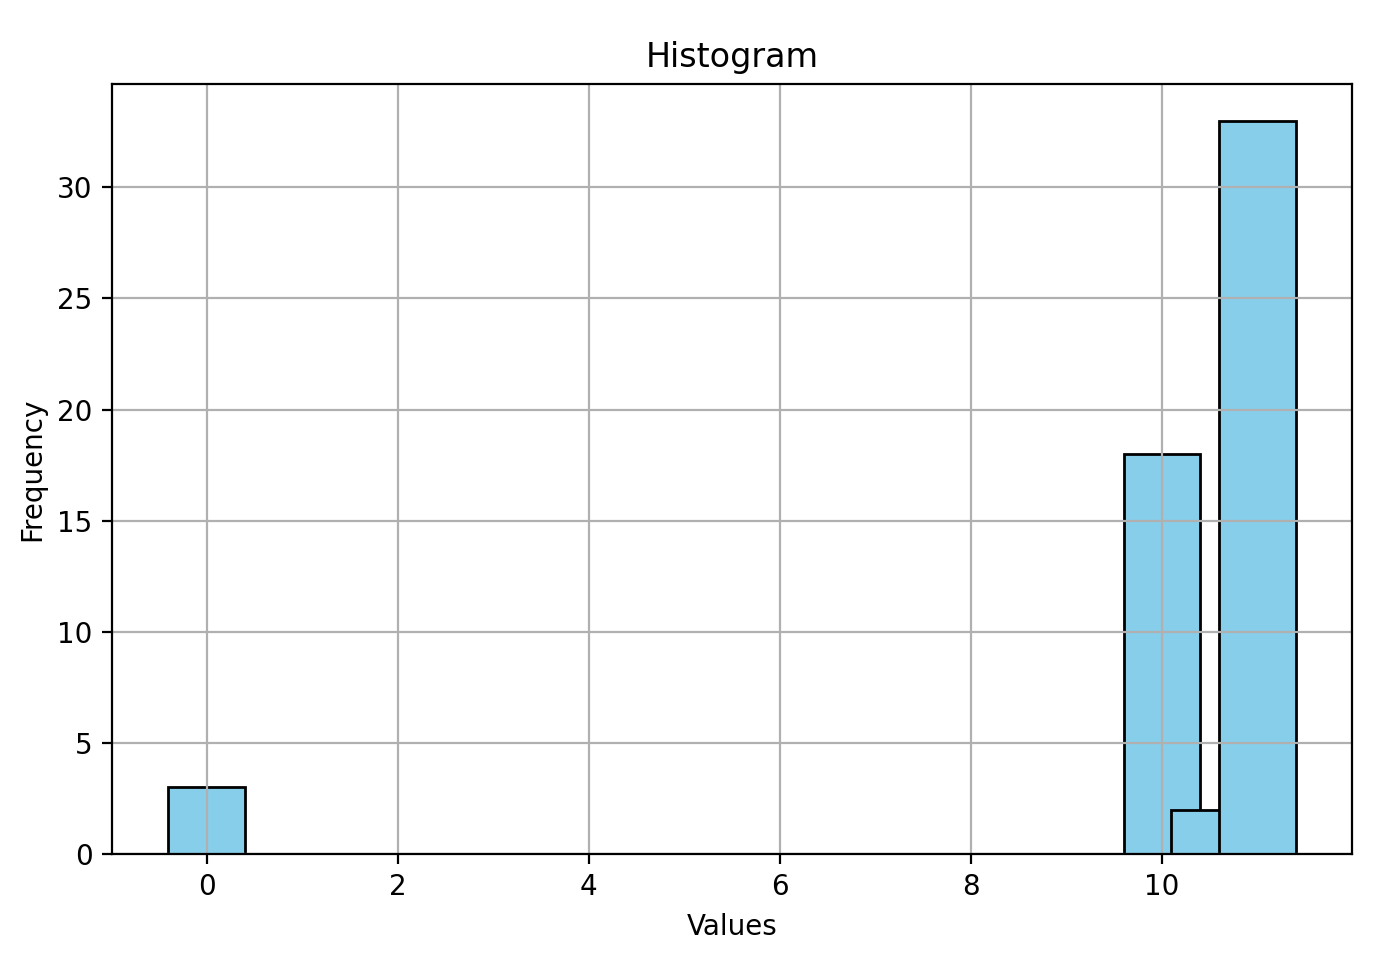
\includegraphics[width=.7\textwidth]{images/reading_quiz_scores}
   		 \caption{Median Score = 11/10 (110\%)}
\end{figure}
\vfill 
\textbf{Rubric.}  	
\begin{itemize}
\item  5 points for correctly answering that the relation WAS a function.
\item 5 points for correct explanation.
\item 1 point EC for additional correct explanation.
\end{itemize}
\end{frame}


\begin{frame}[standout]
Reading Quiz
\end{frame}

\begin{frame}

\begin{mygreenbox}[title= Reading Quiz (Binomial Coefficients)]
\footnotesize 
\begin{enumerate}
	\item Evaluate $\binom{5}{0}$.
	\item Evaluate $\binom{5}{1}$.
	\item (True or False.) $\binom{5}{2} = 1 + 2+ 3+ 4$.
	%\item (True or False.) If $n$ is an integer with $n \geq 2$, then 
	%\[ \binom{n}{2} = 1+ 2+ 3 + \hdots + (n-1) = \sum_{k=1}^{n-1} k. \]
	\item (True or False.) $\binom{5}{3} = \binom{5}{2}$.
	\item (True or False.)  $\binom{n}{2} = \binom{n}{3}$ for any natural number $n$.

	\item (True or False.) Let $n,k \in \mathbb{N}$ with $0 \leq k \leq n$. Then 
	\[ \binom{n}{k} = \binom{n}{n-k} \]
	\item (Extra credit.) Fill in Pascal's Identity below.  Let $n$ and $k$ be integers with $0 < k <n$.  Then 
	\[ \binom{n}{k} = \binom{n-1}{k-1} + \texttt{What?} \]
	\end{enumerate}
\end{mygreenbox}
	
\end{frame}


\begin{frame}[standout]
Q  \& A on Group Exercises  (Functions)
\end{frame}


\begin{frame}[standout]
Overview of binomial coefficients
\end{frame}

\begin{frame}
\footnotesize 
\begin{mygreenbox}[title=Definition of Binomial Coefficient]
Let $n,k \in \mathbb{N}$. The symbol $ \binom{n}{k}$ denotes the number of $k$-element subsets of an $n$-element set.
\end{mygreenbox}

\vfill 


\begin{myredbox}[title=Intepretation]
We can interpret $ \binom{n}{k}$  as the number of \textbf{combinations} when selecting $k$ items from a set of $n$ items.
\end{myredbox}
\vfill 

\begin{myyellowbox}[title=Poll - What is the difference between combinations and permutations?]
\onslide<2->{
\begin{itemize}
\item The number of \textbf{combinations},  $ \binom{n}{k}$, is the number of outcomes when \underline{order doesn't matter}.  We are thinking here in terms of \texttt{sets}. 
\item The number of \textbf{permutations} $(n)_k = n \cdot (n-1) \cdot \hdots \cdot (n-k+1)$, is the number of outcomes where \underline{order matters}.  We are thinking here in terms of \texttt{lists}. 
\end{itemize}
}
\end{myyellowbox}

\onslide<3->{\begin{myredbox}[title=Example]
 Suppose we're making an ice cream sundae. 
 \begin{itemize}
\item Combinations: The selections $(\texttt{M\&M's},\texttt{fudge})= (\texttt{fudge},\texttt{M\&M's})$. 
\item Permutations: The selections $(\texttt{M\&M's},\texttt{fudge}) \neq (\texttt{fudge},\texttt{M\&M's})$. 

\end{itemize}
\end{myredbox}
}
\end{frame}

\begin{frame}{Symmetry}
\footnotesize 
\begin{mygreenbox}[title=Scheinerman Prop 17.7]
Let $n,k \in \mathbb{N}$ with $0 \leq k \leq n$.  Then 
\[ \binom{n}{k} =\binom{n}{n-k} \]
\end{mygreenbox}

\vfill 

\begin{myyellowbox}[title=\text{Poll: What is the intuition?}]
\pause 


\begin{columns}
    \begin{column}{0.7\textwidth}
        \textbf{One answer.} Imagine a class with $n$ children. The teacher has $k$ identical candy bars to give to exactly $k$ children. In how many ways can the $k$ candy bars be distributed?
        \begin{itemize}
            \item The optimist:  $\binom{n}{k} $, because we are selecting $k$ lucky children to get the candy.
            \item The pessimist: 	$\binom{n}{n-k}$, because we are selecting $n-k$ unlucky children to \underline{not} get the candy.
        \end{itemize}
    \end{column}
    \begin{column}{0.25\textwidth}
        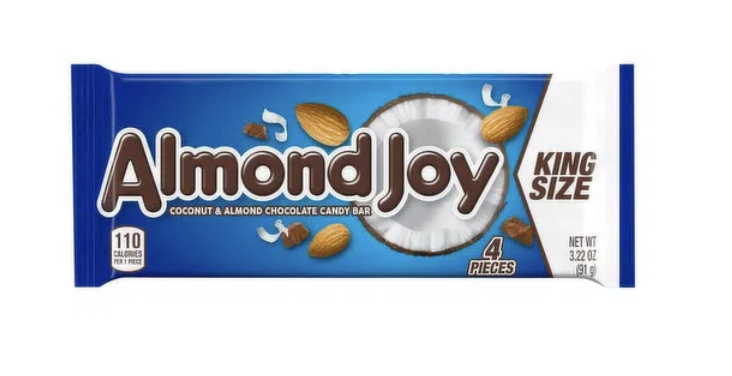
\includegraphics[width=\textwidth]{images/almond_joy}
    \end{column}
\end{columns}
\end{myyellowbox}

\end{frame}


\begin{frame}{Symmetry}
\footnotesize 
\begin{mygreenbox}[title=Scheinerman Prop 17.7]
Let $n,k \in \mathbb{N}$ with $0 \leq k \leq n$.  Then 
\[ \binom{n}{k} =\binom{n}{n-k} \]
\end{mygreenbox}

\vfill 

\begin{myredbox}[title=\text{Example}]
Suppose the class has $n=5$ students and we select $k=2$ students to get candy.  
\vspace{0.15cm}
    Let $A$ be a selection of students who get candy, and $\overline{A}$ be the complementary set (i.e. selection of students who get no candy).  Now note that 
        \begin{itemize}
        \item $\binom{n}{k}=\binom{5}{2}$ is the number of different choices for $A$. 
        \item $\binom{n}{n-k}=\binom{5}{3}$ is the number of different choices for $\overline{A}$. 
        \end{itemize}
		%
     But each possible $A$ is paired up with some $\overline{A}$.  So the number of choices for each must be equal. 
		\begin{center}
        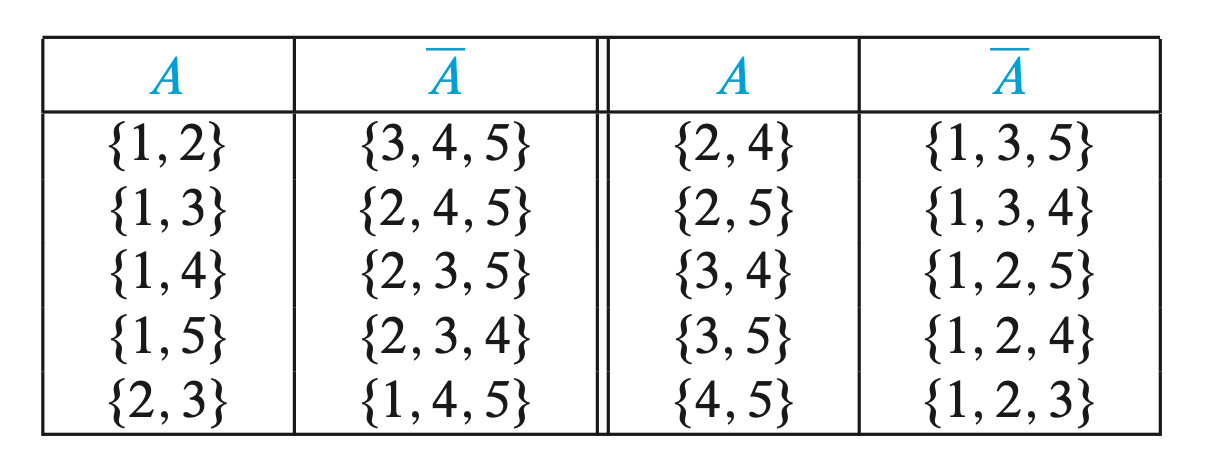
\includegraphics[width=.45\textwidth]{images/symmetry_example}
        \end{center}
\end{myredbox}

\end{frame}


\begin{frame}{Pascal's Triangle}
\footnotesize 
\begin{minipage}{.5\textwidth}
\begin{center}
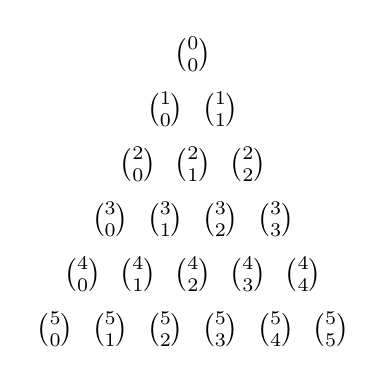
\begin{tikzpicture}[scale=0.7]
\foreach \n in {0,...,5} {
  \foreach \k in {0,...,\n} {
    \node at (\k-\n/2,-\n) {${\n \choose \k}$};
  }
}
\end{tikzpicture}
\end{center}
\end{minipage}
\hfill 
\begin{minipage}{.45\textwidth}
\begin{center}
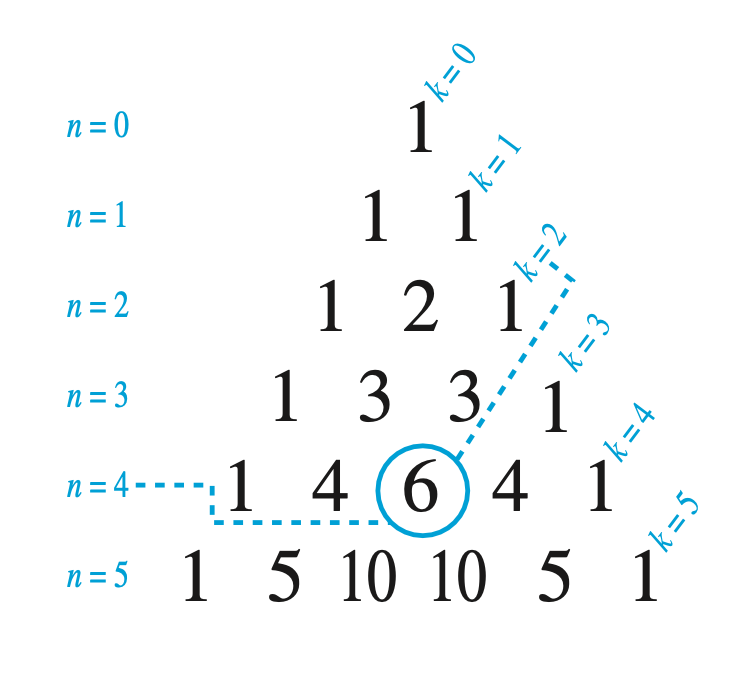
\includegraphics[width=.95\textwidth]{images/pascals_triangle.png}
\end{center}
\end{minipage}

\begin{myredbox}[title=Algorithm for forming Pascal's Triangle]
\begin{itemize}
\item Form an upside-down V shape of 1's. (Why?)
\item The intermediate number in any row is formed by adding the two numbers just to its left and just to its right in the previous row.
\[ \binom{n}{k} =\binom{n-1}{k-1} + \binom{n-1}{k} \]
for integers $k$ and $n$ where $0 < k <n$.
\end{itemize}
\end{myredbox}



\end{frame}


\begin{frame}{Pascal's Triangle}
\footnotesize 
\begin{mygreenbox}[title=\text{Pascal's Identity}]
Let $k$ and $n$ be integers with $0 < k <n$. Then
\[ \binom{n}{k} =\binom{n-1}{k-1} + \binom{n-1}{k} \]
\end{mygreenbox}
\vfill 
\begin{myyellowbox}[title=\text{Poll: What is the intuition?}]
\pause 
Pick one of the elements to be \enquote{weird}. 
\begin{itemize}
\item If we put the weird element in the subset, we have  $\binom{n-1}{k-1}$ ways to complete the subset.
\item If we don't put the weird element in the subset, then we have $ \binom{n-1}{k}$ ways to form the subset.
\end{itemize}

\end{myyellowbox}

\end{frame}


\begin{frame}
\footnotesize 
\begin{mygreenbox}[title=\text{Scheinerman Thm 17.12: \quad Formula for $\binom{n}{k}$}]
Let $k$ and $n$ be integers with $0 \leq  k  \leq n$. Then
\[ \binom{n}{k} = \frac{n!}{k! (n-k)!} \]
\end{mygreenbox}
\vfill 
\begin{myyellowbox}[title=\text{Poll: How to understand this formula?}]
\pause 
\begin{enumerate} \footnotesize 
	\item Suppose we want to select $k$ items from a set of $n$ items, and \underline{order matters}.  Then the number of possible selections is
	%
	\begin{align*}
	(n)_k & = n \cdot (n-1) \cdot \hdots (n-k+1) && \scripttext{(From Sec. 8, Lists)} \\
	&= \frac{n!}{(n-k)!} && \scripttext{(Rewrite using factorial notation)}
	\end{align*}
	\item Now if \underline{order doesn't matter}, we \pause  need to treat all reorderings of the $k$ items as equivalent.  That is, we want to count equivalence classes, each of which has $k!$ members.  So by Scheinerman Theorem 16.6 (Counting equivalence classes), the total number of equivalence classes is $\frac{(n)_k}{k!}$.
\end{enumerate}
\footnotesize 
Hence, 
\[ \binom{n}{k} = \frac{(n)_k}{k!} = \frac{n!}{k! (n-k)!} \]
\end{myyellowbox}

\end{frame}

\begin{frame}{Application: Counting Lattice Paths}
\footnotesize 
\textbf{Problem.} Suppose we want to count the number of grid paths from the lower left corner to the upper right corner in which each step of the path either goes one unit to the right or one unit vertically. How many paths are there?
%
\begin{center}
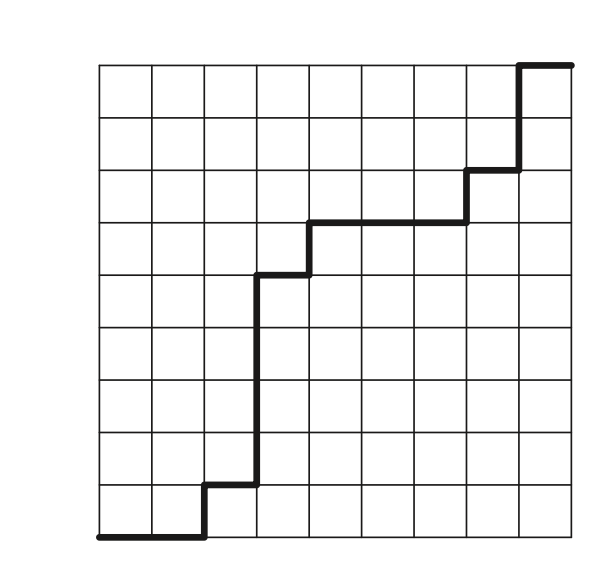
\includegraphics[width=.3\textwidth]{images/lattice_paths.png}
\end{center}
%
\vfill 
\pause 
\textbf{Solution.} Each possible path must take 18 steps - 9 rights and 9 ups.  Using \texttt{R} to denote right and \texttt{U} to denote up, one possible path is
\[\texttt{RRU RUU UUR URR RUR UUR} \]
Now we can count the number of paths by specifying which 9 of the 18 positions have \texttt{R}'s.  The solution is 
\pause 
\[ \binom{18}{9} = 48,620\]
\end{frame}


\begin{frame}[standout]
Group exercises
\end{frame}

\begin{frame}
\footnotesize 
\vfill 
\begin{columns}
\begin{column}{0.33\textwidth}
aaron.loomis: 1 \\ 
adam.wyszynski: 9 \\ 
alexander.goetz: 12 \\ 
alexander.knutson: 12 \\ 
anthony.mann: 9 \\ 
blake.leone: 6 \\ 
bridger.voss: 17 \\ 
caitlin.hermanson: 18 \\ 
cameron.wittrock: 6 \\ 
carsten.brooks: 15 \\ 
carver.wambold: 5 \\ 
colter.huber: 5 \\ 
conner.reed1: 11 \\ 
connor.mizner: 10 \\ 
connor.yetter: 10 \\ 
derek.price4: 11 \\ 
devon.maurer: 2 \\ 
emmeri.grooms: 18 \\ 
erik.moore3: 20 \\ 
ethan.johnson18: 7 \\ 
evan.barth: 4 \\\end{column}
\begin{column}{0.33\textwidth}
evan.schoening: 8 \\ 
griffin.short: 14 \\ 
jack.fry: 17 \\ 
jacob.ketola: 8 \\ 
jacob.ruiz1: 4 \\ 
jacob.shepherd1: 5 \\ 
jada.zorn: 4 \\ 
jakob.kominsky: 16 \\ 
james.brubaker: 3 \\ 
jeremiah.mackey: 8 \\ 
jett.girard: 13 \\ 
john.fotheringham: 13 \\ 
jonas.zeiler: 10 \\ 
joseph.mergenthaler: 14 \\ 
joseph.triem: 3 \\ 
julia.larsen: 20 \\ 
justice.mosso: 19 \\ 
kaden.price: 19 \\ 
lucas.jones6: 1 \\ 
luka.derry: 6 \\ 
luke.donaldson1: 2 \\\end{column}
\begin{column}{0.33\textwidth}
lynsey.read: 15 \\ 
mason.barnocky: 3 \\ 
matthew.nagel: 11 \\ 
micaylyn.parker: 1 \\ 
michael.oswald: 12 \\ 
nolan.scott1: 14 \\ 
owen.obrien: 20 \\ 
pendleton.johnston: 13 \\ 
peter.buckley1: 16 \\ 
reid.pickert: 18 \\ 
ryan.barrett2: 9 \\ 
samuel.hemmen: 21 \\ 
samuel.mosier: 2 \\ 
samuel.rollins: 16 \\ 
sarah.periolat: 21 \\ 
timothy.true: 19 \\ 
tristan.nogacki: 17 \\ 
tyler.broesel: 15 \\ 
william.elder1: 21 \\ 
yebin.wallace: 7 \\ 
zeke.baumann: 7 \\\end{column}
\end{columns}
\vfill
\end{frame}


\begin{frame}{Group exercises}
\footnotesize
\begin{enumerate}
	\item For each question below, determine the answer in three different ways.  First, write out all the possible subsets explicitly.  Second, use a proposition or theorem from the text.  Third, use a different proposition or theorem from the text.  

	\begin{itemize} \footnotesize 
	\item[a.] Determine the number of 2 element subsets of $\set{1,2,3,4,5,6}$.
	\item[b.] Determine the number of 4 element subsets of $\set{1,2,3,4,5,6}$.
	\end{itemize}
	\item Scheinerman Prop 17.7 says: Let $n,k \in \mathbb{N}$ with $0 \leq k \leq n$.  Then 
		\[ \binom{n}{k} = \binom{n}{n-k}. \]
	Prove this proposition using Scheinerman  Theorem 17.12, which says
		\[ \binom{n}{k} = \frac{n!}{k!(n-k)!}. \]
	\item Fifty runners compete in a 5K race.  How many different outcomes are possible? Find different answers according to the context. (a) We want to know in what place every runner finished.  (b) The race is a qualifying race, and we just want to pick the ten fastest runners. (c) The race is an Olympic final event, and we care only about who gets the gold, silver, and bronze medals.
	\item   At a large community festival, there’s a group of 30 volunteers — 8 from Missoula and 22 from other towns. The organizers want to form a five-person team to plan the main event. However, they insist that at least one person from Missoula must be on the team to make sure the town’s voice is heard. How many five-person teams can be formed containing at least one person from Missoula?
	\end{enumerate}

\end{frame}


\begin{frame}{Solution to group exercise \#1a}
\footnotesize

 There are 15 2-elements subsets of $\set{1,2,3,4,5,6}$.  We show this in 3 different ways. 
\begin{enumerate} 
	\item Writing out all the subsets explicitly, we have
%
\begin{align*}
\set{1,2}, \set{1,3}, \set{1,4}, \set{1,5}, \set{1,6} \\
\set{2,3}, \set{2,4}, \set{2,5}, \set{2,6} \\
\set{3,4}, \set{3,5}, \set{3,6} \\
\set{4,5}, \set{4,6} \\
\set{5,6} 
\end{align*}
%
\item The number of subsets of size 2 is given by Scheinerman Prop. 17.5 as 
\[ \binom{n}{2} = \sum_{k=1}^{n-1} k. \]
In this case, since $n=3$, we have $ \binom{6}{2} = 1+2+3=4+5 = 15.$
(Note that the layout of the solution to \#1 suggests why the formula is true.) 
\item The computational formula for $\binom{n}{k}$ (Scheinerman Theorem 17.12) is 
\[ \binom{n}{k}  = \frac{n!}{k! (n-k)!}\] 
Substituting $n=6$ and $k=2$, we find
%
\begin{align*}
\binom{6}{2} = \frac{6!}{2!4!} = \frac{6 \cdot 5}{2 \cdot 1} = 15. 
\end{align*}
\end{enumerate}
\end{frame}

\begin{frame}{Solution to group exercise \#1b}
\footnotesize

 There are 15 4-elements subsets of $\set{1,2,3,4,5,6}$.  We show this in 3 different ways. 
\begin{enumerate} 
	\item Writing out all the subsets explicitly, we have
%
\begin{align*}
\set{3,4,5,6}, \set{2,4,5,6}, \set{2,3,5,6}, \set{2,3,4,6}, \set{2,3,4,5} \\
\set{1,4,5,6}, \set{1,3,5,6}, \set{1,3,4,6}, \set{1,3,4,5} \\
\set{1,2,5,6}, \set{1,2,4,6}, \set{1,2,4,5} \\
\set{1,2,3,6}, \set{1,2,3,5} \\
\set{1,2,3,4} 
\end{align*}
%
\item Scheinerman Prop. 17.7  says that for $n,k \in \mathbb{N}$ with $0 \leq k \leq n$, we have  
\[ \binom{n}{k} = \binom{n}{n-k}\]
Hence  $\binom{6}{4} = \binom{6}{2}$. Since we already know from group exercise \#1a that $\binom{6}{2}=15$, we must have  $\binom{6}{4}=15$. (Indeed, the enumeration of subsets above was obtained by taking the complement of the enumerated subsets from the previous slide.) 
\item The computational formula for $\binom{n}{k}$ (Scheinerman Theorem 17.12) is 
\[ \binom{n}{k}  = \frac{n!}{k! (n-k)!}\] 
Substituting $n=6$ and $k=4$, we find
%
\begin{align*}
\binom{6}{2} = \frac{6!}{4!2!} = \frac{6 \cdot 5}{2 \cdot 1} = 15. 
\end{align*}
\end{enumerate}
\end{frame}

\begin{frame}{Solution to group exercise \#2}
\textbf{Problem.} Scheinerman Prop 17.7 says: Let $n,k \in \mathbb{N}$ with $0 \leq k \leq n$.  Then 
		\[ \binom{n}{k} = \binom{n}{n-k}. \]
	Prove this proposition using Scheinerman  Theorem 17.12. 
\vfill 
\textbf{Solution.} Scheinerman  Theorem 17.12 says
		\[ \binom{n}{k} = \frac{n!}{k!(n-k)!}. \] 
	If we apply Scheinerman  Theorem 17.12 to the problem of finding subsets of size $n-k$ from a set of size $n$, we have
	\[ \binom{n}{n-k} = \frac{n!}{(n-k)!\big(n-(n-k) \big)!} = \frac{n!}{(n-k)!k!} = \frac{n!}{k!(n-k)!}.  \]
Hence,
\[ \binom{n}{k} = \binom{n}{n-k}. \]
			
\end{frame}


\begin{frame}{Solution to group exercise \#3}
\textbf{Problem.}
Fifty runners compete in a 5K race.  How many different outcomes are possible? Find different answers according to the context. (a) We want to know in what place every runner finished.  (b) The race is a qualifying race, and we just want to pick the ten fastest runners. (c) The race is an Olympic final event, and we care only about who gets the gold, silver, and bronze medals.

\vfill 
\textbf{Solution.}
\begin{itemize}
\item[a.] $50!$. Here we want the number of permutations of the 50 runners; that is the number of different ways to order them. 
\item[b.] $\binom{50}{10}$. Here we want to find the number of subsets of size 10 from a pool of size 50.
\item[c.] $\binom{50}{3}$. Here we want to find the number of subsets of size 3 from a pool of size 50.
\end{itemize}
\end{frame}


\begin{frame}{Solution to group exercise \#4}
\small 
\textbf{Problem.}
At a large community festival, there’s a group of 30 volunteers — 8 from Missoula and 22 from other towns. The organizers want to form a five-person team to plan the main event. However, they insist that at least one person from Missoula must be on the team to make sure the town’s voice is heard. How many five-person teams can be formed containing at least one person from Missoula?

\vfill 
\textbf{Solution.}  Let $T$ be the total number of five-person teams.  Let $M$ be the number of five-person teams with at least one person from Missoula.   Let $N$ be the number of five-person teams can with no people from Missoula.  Then
\[ M = T - N. \]

Now $T=\binom{30}{5}$ by definition of the binomial coefficient. (Here we can choose our five-person team from any of the 30 volunteers). Similarly,  $N=\binom{22}{5}$. (Here we must choose our five-person team solely from the 22 volunteers aren't from Missoula). Hence,
\[M = \binom{30}{5} - \binom{22}{5}. \] 


\end{frame}

\end{document}
